\documentclass[12pt]{article}
\usepackage[utf8]{inputenc}
\usepackage{graphicx} % Allows you to insert figures
\usepackage{subcaption}
\usepackage{amsmath} % Allows you to do equations
\usepackage{fancyhdr} % Formats the header
\usepackage{geometry} % Formats the paper size, orientation, and margins
\usepackage{dirtytalk} % typesetting different types of quotation
\usepackage[english]{babel}
\usepackage{csquotes}
\usepackage{hyperref}
\usepackage{listings}
\lstset{
    language=C,
    basicstyle=\ttfamily, 
    numberstyle=\tiny,
    basicstyle=\small,
    frame=single,
    breaklines=true,
    stepnumber=1,                   % the step between two line-numbers.        
    tabsize=2,                      % sets default tabsize to 2 spaces
    breaklines=true,                % sets automatic line breaking
    breakatwhitespace=true,         % sets if automatic breaks should only happen at whitespace
    title=pseudocode
}

\linespread{1.25} % About 1.5 spacing in Word
\setlength{\parindent}{0.8cm} % No paragraph indents
\setlength{\parskip}{0em} % Paragraphs separated by one line
\renewcommand{\headrulewidth}{0pt} % Removes line in header
\geometry{a4paper, portrait, margin=1in}
\setlength{\headheight}{14.49998pt}
\graphicspath{ {images/} }

\begin{document}
\begin{titlepage}
   \begin{center}
    \textsc{\large Ministry of Education of Republic of Moldova}\\[0.5cm]
    \textsc{\large Technical University of Moldova}\\[0.5cm]
    \textsc{\large Faculty of Computers, Informatics and Microelectronics}\\[0.5cm]
    \textsc{\large Software Engineering Department}\\[1.2cm]
    
    \vspace{25 mm}
    
    \textsc{\Large Computer Programming}\\[0.5cm]
    \textsc{\large Laboratory work \#5}\\[0.5cm]    % <<<<<<< CHANGE LAB NUMBER HERE
    
    \newcommand{\HRule}{\rule{\linewidth}{0.5mm}}
    \vspace{10 mm}
    \HRule \\[0.4cm]
    { \LARGE \bfseries Pointers and dynamic memory allocation }\\[0.4cm] % <<<<<<< CHANGE LAB TITLE HERE
    \HRule \\[1.5cm]
    
    \vspace{10mm}
    
    \begin{minipage}[t]{0.4\textwidth}
    \begin{flushleft} \large
    \emph{Author:} \\
    Andrei \textsc{Chicu}\\                         % <<<<<<< CHANGE YOUR NAME HERE
    std. gr. FAF-233                                % <<<<<<< CHANGE GROUP NUMBER HERE
    \end{flushleft}
    \end{minipage}
    ~
    \begin{minipage}[t]{0.4\textwidth}
    \begin{flushright} \large
    \emph{Verified:} \\
    Alexandru \textsc{Furdui}\\
    \end{flushright}
    \end{minipage}\\[3cm]
    
    \vspace{5 mm}
    \large Chișinău 2023\\[0.5cm]
    
    \vfill
    \end{center}
\end{titlepage}

\setcounter{page}{2}
\pagestyle{fancy}
\fancyhf{}
\rhead{\thepage}
\lhead{FAF-233 Andrei Chicu; Laboratory Work №5}

% \section*{Introduction}
\section*{Theory Background}
A stack data structure[\ref{plist}], often denoted as \textbf{LIFO} (Last In, First Out), is a linear data structure in computer science. It can be thought of as a collection of elements with two main operations: \texttt{push()}, which adds an element to the top of the stack, and \texttt{pop()}, which removes the top element.

Dynamic memory allocation in C refers to the process of allocating and deallocating memory for data structures at runtime. The functions \texttt{malloc()}, \texttt{calloc()}, and \texttt{realloc()} are commonly used in C to allocate memory dynamically. This allows programs to allocate memory as needed, rather than having fixed, compile-time memory allocations. Proper management of dynamically allocated memory is crucial to prevent memory leaks and optimize resource usage in C programs.

In the program of this project, users can interact with it through a command-line interface, allowing them to perform essential stack operations, including push, pop, peek, and check for stack status (empty or full), making it easier to create stack-based data structures while handling various data types.

The program takes advantage of \texttt{void*} pointers to store data of various datatypes avoiding the use of structures such as unions.

\section*{The Task}
\emph{Task Hard}. Implement a Stack Data Structure with Dynamic Memory Allocation.

\section*{Technical implementation}
The full code is at \url{https://github.com/andyp1xe1/pc_labs/tree/master/lab5}
\begin{lstlisting}
// define constants for data types
enum type_t:
  of_int
  of_float
  of_char
  of_string

// define a node structure
struct node_t:
  type: type_t
  data: pointer
  next: pointer

// define a stack structure
struct stack_t:
  node: pointer to node_t
  size: integer
  nnum: integer

// function to print a node
function print_node(node: pointer to node_t):
  p = node.data
  switch node.type:
    case of_int:
      print "p->data: ", p as integer
    case of_float:
      print "p->data: ", p as float
    case of_char:
      print "p->data: ", p as char
    case of_string:
      print "p->data: ", p as string

// function to free a node
function free_node(node: pointer to node_t):
  if node is not null:
    free(node)

// function to allocate data based on type
function alloc_data_of(type: type_t):
  switch type:
    case of_int:
      return allocate memory for an integer
    case of_float:
      return allocate memory for a float
    case of_char:
      return allocate memory for a char
    case of_string:
      return allocate memory for a string

// function to initialize a node
function init_node(type: type_t):
  node = allocate memory for a node_t
  if node is null:
    return null
  node.type = type
  node.data = alloc_data_of(type)
  node.next = null
  return node

// function to copy data from source to destination
function copy_data(dest: pointer, source: pointer, type: type_t):
  size = size of data based on type
  copy data from source to dest with the specified size

// function to check if the stack is full
function is_full(stack: pointer to stack_t):
  if stack.size equals stack.nnum:
    return 1
  else:
    return 0

// function to check if the stack is empty
function is_empty(stack: pointer to stack_t):
  if stack.node is null:
    return 1
  else:
    return 0

// function to push data onto the stack
function push(stack: pointer to stack_t, data: pointer, type: type_t):
  to_add = init_node(type)
  if to_add is null:
    free(to_add)
    print "no space left for allocating"
    return 0
  copy_data(to_add.data, data, type)
  to_add.next = stack.node
  stack.node = to_add
  stack.nnum++
  return 1

// function to pop data from the stack
function pop(stack: pointer to stack_t):
  to_remove = stack.node
  if stack.node is null:
    return null
  stack.node = stack.node.next
  return to_remove

// function to handle push operation
function handle_push(stack: pointer to stack_t):
  t as char
  r as integer
  if stack.size equals stack.nnum:
    print "stack is full"
    return
  print "choose type:"
  print "(i)nteger"
  print "(f)loat"
  print "(c)har"
  print "(s)tring"
  print "type: "
  read t
  print "data:"
  switch t:
    case 'i':
      data as integer
      read data
      r = push(stack, &data, of_int)
    case 'f':
      data as float
      read data
      r = push(stack, &data, of_float)
    case 'c':
      data as char
      read data
      r = push(stack, &data, of_char)
    case 's':
      data as string
      read data
      r = push(stack, data, of_string)
  if r:
    print "pushed element successfully"
  else:
    print "failed to push"

// function to handle pop operation
function handle_pop(stack: pointer to stack_t):
  n = pop(stack)
  if n is not null:
    print "popped element successfully"
    print_node(n)
    free(n.data)
    free(n)
  else:
    print "stack is empty"

// function to run the REPL (Read-Eval-Print Loop)
function repl(stack: pointer to stack_t):
  o as char
  sz as integer
  while stack.size <= 0:
    print "enter size of stack: "
    read sz
    if sz <= 0:
      print "size should be positive"
    else:
      stack.size = sz
  print "type 'h' for help"
  repeat:
    print "-> "
    read o
    switch o:
      case 'h':
        print "commands:"
        print "'h': display this message"
        print "'+': push an item"
        print "'-': pop and display the top item"
        print "'p': peek at the top item"
        print "'e': check if empty"
        print "'f': check if full"
        print "'!': exit"
      case '+':
        handle_push(stack)
        print "stack size: ", stack.size
      case '-':
        handle_pop(stack)
        print "stack size: ", stack.size
      case 'p':
        if is_empty(stack):
          print "stack is empty"
        else:
          print_node(stack.node)
      case 'e':
        if is_empty(stack):
          print "stack is empty"
        else:
          print "stack is not empty"
      case 'f':
        if is_full(stack):
          print "stack is full"
        else:
          print "stack is not full"
      case '!':
        return

// main function
function main():
  stack as pointer to stack_t
  stack = allocate memory for a stack_t
  stack.node = null
  stack.size = 0
  repl(stack)
  n as pointer to node_t
  repeat:
    n = pop(stack)
    if n is not null:
      free(n.data)
      free(n)
  free(stack)
  return exit_success
\end{lstlisting}

\pagebreak
\section*{Results}
\hspace{0.8cm}
here is a little demo of the stack:
\begin{figure}[!h]
  \centering
  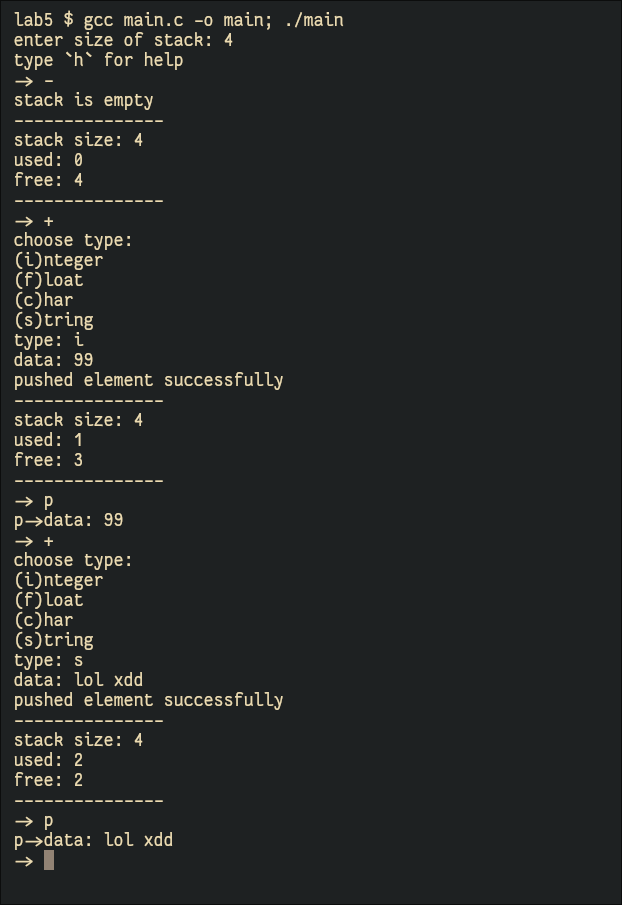
\includegraphics[width=5in]{stack_demo.png}
  \caption{stack demo}
\end{figure}
\pagebreak

\section*{Conclusion}
\hspace{0.8cm}
In summary, the C program I wrote demonstrates the implementation of dynamic memory allocation and linked lists for a stack data structure. It offers flexibility by supporting different data types, such as integers, floats, characters, and strings. The code effectively manages memory allocation and deallocation, ensuring proper memory usage during push and pop operations.

Also, it provides a solid foundation for understanding and working with dynamic memory allocation and linked lists in C.

\section*{Bibliography}
\hspace{0.8cm}
\begin{enumerate}
    \item  \label{plist} \url{https://www.youtube.com/playlist?list=PLfqABt5AS4FmXeWuuNDS3XGENJO1VYGxl}
    \item \url{https://stackoverflow.com/questions/40681151/what-happens-to-scanf-if-the-entered-value-from-a-file-is-empty}
    \item \url{https://duckduckgo.com/?t=ffab&q=copy+memory+between+void+pointers}
\end{enumerate}

\pagebreak
\end{document}
